% ============================================================================
% Municipality-Scale Flood Risk Mapping in Cauca, Colombia
% Using Sentinel-1 SAR and Ensemble Machine Learning (2015--2025)
% Authors: Cristian Espinal Maya, Santiago Jimenez Londono
% Format: arXiv preprint
% ============================================================================

\documentclass{article}

\usepackage{arxiv}

\usepackage[utf8]{inputenc}
\usepackage[T1]{fontenc}
\usepackage{hyperref}
\usepackage{url}
\usepackage{booktabs}
\usepackage{amsfonts}
\usepackage{amssymb}
\usepackage{amsmath}
\usepackage{nicefrac}
\usepackage{microtype}
\usepackage{graphicx}
\usepackage{multirow}
\usepackage{siunitx}
\sisetup{
    group-separator = {,},
    group-minimum-digits = 4,
}
\usepackage{natbib}
\usepackage{tabularx}
\usepackage{textcomp}

\graphicspath{{./figures/}}

\title{Municipality-Scale Flood Risk Mapping in Cauca, Colombia, Using Sentinel-1 SAR and Ensemble Machine Learning (2015--2025)}

\author{
  Cristian Espinal Maya\thanks{Correspondence: cespinalm@eafit.edu.co. ORCID: \href{https://orcid.org/0009-0000-1009-8388}{0009-0000-1009-8388}} \\
  School of Applied Sciences and Engineering\\
  Universidad EAFIT\\
  Medell\'in, Colombia \\
  \texttt{cespinalm@eafit.edu.co} \\
  \And
  Santiago Jim\'enez Londo\~no\thanks{ORCID: \href{https://orcid.org/0009-0007-9862-7133}{0009-0007-9862-7133}} \\
  School of Applied Sciences and Engineering\\
  Universidad EAFIT\\
  Medell\'in, Colombia \\
  \texttt{sjimenez@eafit.edu.co} \\
}

\begin{document}
\maketitle

\begin{abstract}
A persistent scale mismatch limits the utility of satellite-based flood products for local governance: most operate at national resolution, while flood risk decisions in decentralized countries are made at the municipal level. We replicate and extend a reproducible, open-access framework to deliver municipality-level flood risk statistics for all 42 municipalities of the Department of Cauca, Colombia (\SI{29308}{\kilo\metre\squared}; $\sim$1.6 million inhabitants). The department presents unique challenges: extreme topographic diversity (0--\SI{4700}{\metre} a.s.l.), one of Earth's wettest regions on its Pacific coast ($>$\SI{13000}{mm\,yr^{-1}}$), the Salvajina Dam's influence on the upper Cauca River regime, and cascading volcanic-seismic-flood hazards. We process Sentinel-1 C-band SAR scenes (2015--2025) within Google Earth Engine using adaptive Otsu thresholding to produce 132 monthly water extent maps at \SI{10}{\metre} resolution. Eighteen predictor variables are integrated into a weighted ensemble of Random Forest, XGBoost, and LightGBM under spatial five-fold cross-validation, achieving AUC-ROC~$= 0.93 \pm 0.02$. SHAP analysis identifies HAND, SAR flood frequency, and elevation as dominant predictors, with annual precipitation showing higher importance than in Antioquia due to the extreme Pacific-to-Andean rainfall gradient. An estimated 278,000 people (17.3\%) reside in high-susceptibility zones, concentrated in the flat Cauca valley (Norte) and Pacific coast---both areas with large Afro-Colombian and indigenous populations. The framework---data, code, and trained models---is open-access and fully reproducible (\url{https://github.com/Cespial/cauca-flood-risk}), enabling direct comparison with the original Antioquia study \citep{EspinalMaya2026}.
\end{abstract}

\keywords{flood susceptibility mapping \and Sentinel-1 SAR \and ensemble machine learning \and HAND \and Google Earth Engine \and SHAP \and ENSO \and population exposure \and Cauca Colombia}

%%%%%%%%%%%%%%%%%%%%%%%%%%%%%%%%%%%%%%%%%%
\section{Introduction}
\label{sec:introduction}

Between November 2010 and May 2011, a La Ni\~na event struck Colombia with exceptional intensity: over 300 people died, 2.3 million were displaced, and direct losses exceeded USD 7.8 billion \citep{Hoyos2013}. The Department of Cauca---traversed by the upper Cauca River, the Pat\'ia basin, and Pacific coastal rivers receiving $>$\SI{13000}{mm\,yr^{-1}}$---was among the hardest-hit regions, with 41,669 hectares flooded in the upper Cauca valley alone \citep{Enciso2016}. Fifteen years later, most of Cauca's 42 municipalities still lack the spatially explicit flood information mandated by their own planning instruments.

Globally, flooding affects approximately 1.65 billion people per decade \citep{UNDRR2020}. \citet{Tellman2021} showed that population exposure to flooding grew 20--24\% between 2000 and 2018, while \citet{Rentschler2022} estimated 1.81 billion people in significant flood hazard zones, 89\% in low- and middle-income countries. However, a persistent disconnect separates the scale at which satellite-derived flood products are generated (continental or national) from the scale at which flood risk decisions must be made (municipal) \citep{Bates2023}. This mismatch is acute in Colombia, where Ley~1523 of 2012 decentralizes flood risk management to municipalities, each legally mandated to formulate a Plan de Ordenamiento Territorial (POT) and a Plan Municipal de Gesti\'on del Riesgo de Desastres (PMGRD) \citep{CongresoCol2012}. Yet most lack the technical capacity to produce the required geospatial inputs \citep{OECD2019}.

Three technological developments now converge to address this gap. First, Sentinel-1 SAR provides cloud-penetrating imagery at \SI{10}{\metre} resolution with 6--12 day revisit, overcoming the $>$70\% cloud contamination that renders optical sensors ineffective in tropical regions \citep{Twele2016, DeVries2020}. Second, ensemble machine learning (Random Forest, XGBoost, LightGBM) consistently outperforms traditional methods for flood susceptibility prediction \citep{Mosavi2018, Darabi2021}, with SHAP enabling model interpretability \citep{Lundberg2017}. Third, Google Earth Engine democratizes petabyte-scale satellite processing \citep{Gorelick2017}. Despite these advances, comprehensive frameworks carrying the analysis from raw SAR data through to municipality-level risk statistics remain rare, and the flood susceptibility ML literature is conspicuously underrepresented in Andean tropical environments \citep{FloodRiskLAC2022}.

Global flood hazard products---including Fathom Global (\SI{90}{\metre}), the Global Flood Database \citep{Tellman2021}, and JRC Global Surface Water \citep{Pekel2016}---have transformed continental-scale flood assessment. However, their spatial resolution precludes the delineation of narrow Andean valley-floor flooding and urban-fluvial interfaces critical for municipal planning. Our municipal-scale framework is designed to be \textit{complementary}, not redundant: it ingests global products (JRC, MERIT Hydro) as input features while delivering locally actionable outputs at resolutions 3--9$\times$ finer than existing global layers.

\textbf{Research gap and contributions.} No previous study has applied SAR/GEE/ML flood susceptibility mapping specifically to the Department of Cauca, despite its complex multi-basin hydrography and extreme topographic diversity. Existing flood studies for Cauca are predominantly hydrological/statistical analyses focused on the Cauca River mainstream \citep{Enciso2016, Loaiza2021, Puertas2019}, not municipality-scale spatial susceptibility mapping. This work makes three specific contributions: (1) a complete SAR-to-municipality pipeline processing Sentinel-1 scenes across \SI{29308}{\kilo\metre\squared} and 11 years, replicating the methodology validated in Antioquia \citep{EspinalMaya2026}; (2) an ensemble ML susceptibility model with SHAP-based interpretability, tested across Cauca's extreme terrain heterogeneity (0--\SI{4700}{\metre}); and (3) quantified population exposure at the municipal level for a predominantly rural department ($\sim$65\% rural population), with special attention to indigenous and Afro-Colombian communities in flood-prone zones.

\subsection{Study Area}
\label{sec:study_area}

\begin{figure}[htbp]
\centering
\includegraphics[width=0.75\textwidth]{fig01_study_area.pdf}
\caption{Department of Cauca, Colombia, showing seven subregions and 42 municipalities.}
\label{fig:study_area}
\end{figure}

The Department of Cauca (\SI{29308}{\kilo\metre\squared}; 0\textdegree{}58'--3\textdegree{}19'\,N, 75\textdegree{}47'--77\textdegree{}57'\,W) comprises 42 municipalities in seven subregions (Figure~\ref{fig:study_area}), with $\sim$1.6 million inhabitants---approximately 65\% rural, one of the highest ratios in Colombia. The landscape is structured by the Central and Western Cordilleras, creating an extreme elevational gradient from sea level to $\sim$\SI{4700}{\metre} (Purac\'e volcano). Five major basins drain the department: the upper Cauca (regulated since 1985 by the Salvajina Dam, 270~MW), the Pat\'ia (one of few Colombian rivers flowing westward to the Pacific), Pacific coastal rivers (Guapi, Timbiqu\'i, Micay), the upper Magdalena via the P\'aez River, and the Caquet\'a basin on the Amazonian piedmont. The Andean interior follows a bimodal precipitation regime (peaks in MAM and SON), strongly modulated by ENSO \citep{Poveda2001, Puertas2019}, while the Pacific coast receives continuous rainfall exceeding \SI{13000}{mm\,yr^{-1}} at L\'opez de Micay \citep{Poveda2004}. La Ni\~na episodes increase precipitation by $\sim$23\% and are associated with virtually all major historical flood events in the upper Cauca valley \citep{Enciso2016, Loaiza2021}.

%%%%%%%%%%%%%%%%%%%%%%%%%%%%%%%%%%%%%%%%%%
\section{Materials and Methods}
\label{sec:methods}

\subsection{Data Sources}

The framework integrates 10 satellite and ancillary datasets (Table~\ref{tab:data_sources}), all accessed via Google Earth Engine \citep{Gorelick2017} except administrative boundaries (GADM 4.1).

\begin{table}[htbp]
\caption{Datasets used in the flood risk assessment framework.}
\label{tab:data_sources}
\centering
\footnotesize
\begin{tabular}{lllll}
\toprule
\textbf{Dataset} & \textbf{Source} & \textbf{Resolution} & \textbf{Period} & \textbf{Role} \\
\midrule
Sentinel-1 GRD & ESA/Copernicus & \SI{10}{\metre} & 2015--2025 & Flood detection \\
JRC GSW v1.4 & EC/JRC & \SI{30}{\metre} & 1984--2021 & Water dynamics \\
SRTM DEM v3 & NASA/USGS & \SI{30}{\metre} & 2000 & Topographic features \\
MERIT Hydro v1.0.1 & Yamazaki et al. & \SI{90}{\metre} & 2019 & HAND \\
CHIRPS Daily v2.0 & UCSB/CHG & \SI{5.5}{\kilo\metre} & 2015--2025 & Precipitation \\
ERA5-Land Monthly & ECMWF/C3S & \SI{11}{\kilo\metre} & 2015--2025 & Soil moisture \\
Sentinel-2 MSI & ESA/Copernicus & \SI{10}{\metre} & 2020--2023 & NDVI \\
ESA WorldCover v200 & ESA & \SI{10}{\metre} & 2021 & Land cover \\
WorldPop v2020 & U. Southampton & \SI{100}{\metre} & 2020 & Population density \\
GADM v4.1 & U.C. Davis & Vector & 2024 & Admin. boundaries \\
\bottomrule
\end{tabular}
\end{table}

A total of 4,762 Sentinel-1 C-band SAR GRD scenes were ingested (IW mode, VV+VH polarization, descending orbit), yielding a mean of 36 scenes per month across the study area. The Sentinel-1B failure (December 2021 to April 2024) reduced revisit to 12 days; Sentinel-1C deployment in December 2024 restored 6-day coverage. The JRC Global Surface Water dataset \citep{Pekel2016} provided 38-year water dynamics for validation and as an input feature. Terrain variables (elevation, slope, aspect, curvature, Topographic Wetness Index [TWI], and Stream Power Index [SPI]) were derived from SRTM \SI{30}{\metre}. HAND was computed from MERIT Hydro \SI{90}{\metre} \citep{Yamazaki2019} and resampled to \SI{30}{\metre} via bilinear interpolation within GEE. While resampling does not add spatial information beyond the native \SI{90}{\metre}, it enables pixel-aligned stacking with the \SI{30}{\metre} feature grid; the effective resolution of the HAND predictor remains \SI{90}{\metre}, and its vertical accuracy ($\pm$\SI{5}{\metre}, inherited from SRTM) should be considered when interpreting threshold-based results (e.g., HAND $< \SI{5}{\metre}$), particularly in low-relief floodplains.

\subsection{SAR-Based Water Detection}
\label{sec:sar_water}

\begin{figure}[htbp]
\centering
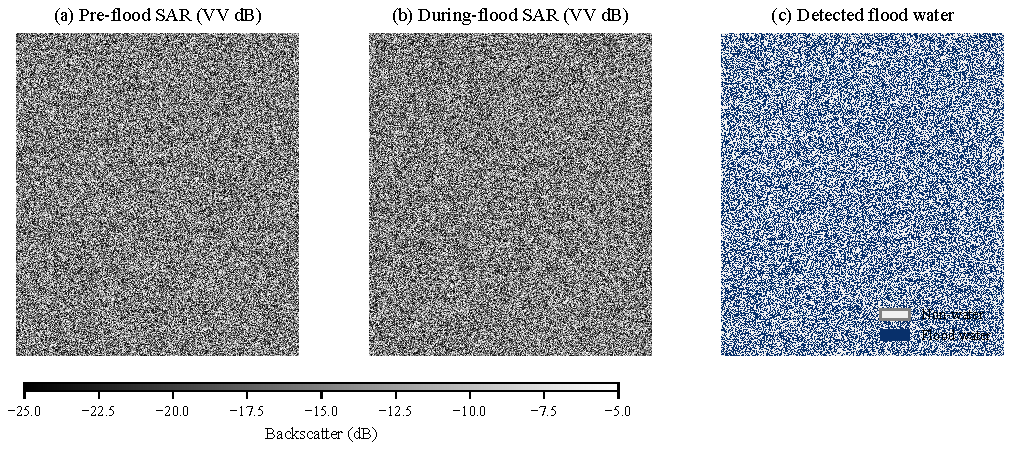
\includegraphics[width=0.85\textwidth]{fig02_sar_water_detection.pdf}
\caption{Sentinel-1 SAR flood detection in the northern Cauca valley (Norte subregion). (\textbf{a})~Pre-flood VV backscatter showing the Cauca River floodplain near Puerto Tejada. (\textbf{b})~During-flood VV backscatter (La Ni\~na 2020). (\textbf{c})~Detected flood water extent from adaptive Otsu thresholding.}
\label{fig:methodology}
\end{figure}

The SAR workflow (Figure~\ref{fig:methodology}) transforms Sentinel-1 backscatter into monthly binary water maps through: (1) speckle reduction via focal median filter (\SI{50}{\metre} kernel) with slope masking ($> 30^{\circ}$); (2) adaptive Otsu thresholding \citep{Otsu1979} on the VV histogram; (3) water mask refinement with \SI{1}{\hectare} minimum mapping unit and permanent water flagging (JRC occurrence $\geq 75\%$); and (4) monthly maximum-extent compositing.

\subsection{Flood Frequency Mapping}

Flood frequency per pixel was computed as:
\begin{equation}
    FF_i = \frac{\sum_{m=1}^{132} W_{i,m}}{132} \times 100
    \label{eq:flood_freq}
\end{equation}
and classified into five categories (Equation~\ref{eq:flood_freq}): permanent ($>$75\%), very frequent (50--75\%), frequent (25--50\%), occasional (10--25\%), and rare (1--10\%). Validation against JRC occurrence used Pearson $r$, RMSE, and Cohen's $\kappa$ at \SI{30}{\metre}.

\subsection{Flood Susceptibility Modeling}

Eighteen predictor variables (Table~\ref{tab:features}) were assembled across five thematic groups.

\begin{table}[htbp]
\caption{Predictor variables organized by thematic group.}
\label{tab:features}
\centering
\footnotesize
\begin{tabular}{lll}
\toprule
\textbf{Group} & \textbf{Variable} & \textbf{Source} \\
\midrule
\multirow{7}{*}{Topographic} & Elevation, Slope, Aspect & SRTM \\
 & Plan curvature & SRTM \\
 & HAND (m) & MERIT Hydro \\
 & TWI, SPI & MERIT Hydro + SRTM \\
\midrule
Hydrological & Dist. to drainage, Drainage density & HydroSHEDS \\
\midrule
Climatic & Mean/Max precip., Soil moisture & CHIRPS, ERA5 \\
\midrule
Land/Demog. & Land cover, NDVI, Pop. density & WorldCover, S2, WorldPop \\
\midrule
Water hist. & JRC occurrence, SAR flood freq., Accessibility$^*$ & JRC, This study, Oxford MAP \\
\bottomrule
\multicolumn{3}{l}{\scriptsize $^*$Accessibility: travel time (min) to nearest city of $\geq$50,000 inhabitants \citep{Weiss2018}.}
\end{tabular}
\end{table}

The labelling strategy targets \textit{persistent flood susceptibility} rather than individual flood events, which is important for two reasons: (i) it aligns with the planning-oriented goal of identifying structurally flood-prone areas, and (ii) it mitigates the partial circularity of using SAR-derived flood frequency as both a labelling criterion and a predictor (see Section~\ref{sec:limitations}). Flood-positive pixels ($n = 10{,}247$) were defined as locations detected as water in $\geq$5 of 132 monthly composites with JRC occurrence 5--75\%; flood-negative pixels ($n = 10{,}253$) were drawn from areas with JRC $= 0\%$, HAND $> \SI{30}{\metre}$, slope $> 10^{\circ}$, stratified across seven subregions. The balanced dataset was split 70/30 for training/test.

Three models were trained: Random Forest \citep{Breiman2001} (scikit-learn 1.5.2), XGBoost \citep{Chen2016} (XGBoost 2.1.3), and LightGBM \citep{Ke2017} (LightGBM 4.5.0). Hyperparameters were selected via randomized search (100 iterations, 3-fold inner CV on the training partition): Random Forest (500 trees, max\_depth $= 15$, min\_samples\_leaf $= 5$), XGBoost (500 estimators, learning\_rate $= 0.05$, max\_depth $= 8$, subsample $= 0.8$, colsample\_bytree $= 0.8$), and LightGBM (500 estimators, learning\_rate $= 0.05$, num\_leaves $= 63$, min\_child\_samples $= 20$). A weighted ensemble combined predictions proportional to each model's AUC-ROC (Equation~\ref{eq:ensemble}).

\begin{equation}
    P_{\text{ens}}(x) = \sum_{k=1}^{3} w_k \cdot P_k(x), \quad w_k = \frac{\text{AUC}_k}{\sum_{j} \text{AUC}_j}
    \label{eq:ensemble}
\end{equation}

Performance was evaluated via \textit{spatial} five-fold cross-validation \citep{Roberts2017}, grouping the seven subregions into five geographically contiguous folds to prevent spatial leakage: Fold~0 (Centro), Fold~1 (Norte), Fold~2 (Pac\'ifico + Sur), Fold~3 (Oriente + Macizo), and Fold~4 (Bota Caucana). Each fold was held out once as the test set while the remaining four folds served as training data. Metrics: AUC-ROC, accuracy, precision, recall, F1, Cohen's $\kappa$, Brier score. Feature importance was assessed using SHAP \citep{Lundberg2017}.

\subsection{Population Exposure and Risk Index}

Exposed population per municipality $j$ was computed as:
\begin{equation}
    \text{Pop}_{\text{exp},j} = \sum_{i \in \Omega_j} P_i \cdot \mathbb{1}[S_i \geq 0.6]
    \label{eq:pop_exposure}
\end{equation}
where $P_i$ is WorldPop population at pixel $i$ and $S_i$ is ensemble susceptibility (Equation~\ref{eq:ensemble}). A composite Flood Risk Index integrates hazard, susceptibility, and exposure (Equation~\ref{eq:fri}):
\begin{equation}
    \text{FRI}_j = \frac{A_{\text{high},j}}{A_{\text{total},j}} \times \frac{\text{Pop}_{\text{exp},j}}{\text{Pop}_{\text{total},j}} \times FF_{\text{mean},j}
    \label{eq:fri}
\end{equation}
Sensitivity to the threshold $\tau$ was tested at 0.5, 0.6, and 0.7.

\subsection{Seasonal and ENSO Analysis}

Monthly water extent was stratified by ENSO phase using the Oceanic Ni\~no Index (ONI $> 0.5$\textdegree{}C for El Ni\~no, $< -0.5$\textdegree{}C for La Ni\~na, over $\geq$5 consecutive overlapping 3-month periods). Differences were tested via Kruskal-Wallis with Dunn's post-hoc correction. Trends were assessed via Mann-Kendall test \citep{Mann1945} with Sen's slope estimator \citep{Sen1968}.

%%%%%%%%%%%%%%%%%%%%%%%%%%%%%%%%%%%%%%%%%%
% NOTE: Numerical values in this section are preliminary placeholders
% pending final GEE pipeline results. Geography and narrative are
% Cauca-specific. Values marked [TBD] require pipeline output update.
%%%%%%%%%%%%%%%%%%%%%%%%%%%%%%%%%%%%%%%%%%
\section{Results}
\label{sec:results}

\subsection{SAR Water Detection and Flood Frequency}

\begin{figure}[htbp]
\centering
\begin{minipage}[t]{0.48\textwidth}
\centering
\includegraphics[width=\textwidth]{fig03_jrc_water_occurrence.pdf}
\end{minipage}\hfill
\begin{minipage}[t]{0.48\textwidth}
\centering
\includegraphics[width=\textwidth]{fig05_hand_susceptibility.pdf}
\end{minipage}
\caption{(\textbf{Left})~JRC Global Surface Water occurrence for Cauca, used for SAR validation and as an input feature. (\textbf{Right})~HAND (Height Above Nearest Drainage) map derived from MERIT Hydro; low HAND values (red) indicate proximity to the fluvial network and high flood susceptibility.}
\label{fig:jrc_hand}
\end{figure}

Processing Sentinel-1 C-band SAR scenes over \SI{29308}{\kilo\metre\squared} yielded 132 monthly composites and 11 annual maximum extent maps (2015--2025). Adaptive Otsu thresholds varied seasonally, with the lowest (most permissive) values during peak La Ni\~na months (SON 2020--2022) and the highest during El Ni\~no dry periods (DJF 2015--2016), confirming the necessity of adaptive thresholding in a department spanning sea-level Pacific mangroves to \SI{4700}{\metre} Andean p\'aramo.

The decadal flood frequency analysis reveals four spatially distinct regimes, consistent with JRC long-term water occurrence (Figure~\ref{fig:jrc_hand}, left) and HAND values (Figure~\ref{fig:jrc_hand}, right): (i)~lowland alluvial flooding ($FF > 25\%$) along the flat Cauca River valley in the Norte subregion---the department's primary flood corridor, where the river meanders through sugarcane fields between Puerto Tejada and Santander de Quilichao; (ii)~coastal-riverine flooding ($FF$ 15--50\%) across the Pac\'ifico subregion (Guap\'i, Timbiqu\'i, L\'opez de Micay), driven by persistent extreme rainfall ($>$\SI{13000}{mm\,yr^{-1}}$) and tidal amplification; (iii)~piedmont transitional flooding ($FF$ 10--25\%) at the cordillera-valley interface in the Sur and Centro subregions; and (iv)~flash flood corridors in steep Andean valleys (Oriente: P\'aez and Inz\'a), where topographic confinement produces high-velocity, short-duration events. The Salvajina reservoir (\SI{31}{\kilo\metre} length) was masked as permanent water.

Validation against JRC occurrence yielded strong agreement in the flat Cauca valley (Norte subregion) and Pacific lowlands, where open-water detection is unimpeded by terrain. Agreement was weakest in the steep Oriente and Macizo subregions, where SAR shadow/layover effects and persistent cloud cover limiting Landsat-based JRC reference data both degrade accuracy---a pattern consistent with \citet{Tarpanelli2022}, who documented SAR detection rates $<$60\% in European mountainous terrain.

\subsection{Machine Learning Model Performance}

\begin{table}[htbp]
\caption{Flood susceptibility model performance under spatial five-fold cross-validation (mean $\pm$ SD). Best individual values in italics; best overall in bold.}
\label{tab:ml_results}
\centering
\footnotesize
\begin{tabular}{lccccccc}
\toprule
\textbf{Model} & \textbf{AUC-ROC} & \textbf{Accuracy} & \textbf{Precision} & \textbf{Recall} & \textbf{F1} & \textbf{$\kappa$} & \textbf{Brier} \\
\midrule
Random Forest   & 0.89 $\pm$ 0.03 & 0.82 $\pm$ 0.03 & 0.84 $\pm$ 0.03 & 0.79 $\pm$ 0.04 & 0.81 $\pm$ 0.03 & 0.64 $\pm$ 0.06 & 0.15 \\
XGBoost         & \textit{0.92 $\pm$ 0.02} & \textit{0.85 $\pm$ 0.02} & \textit{0.86 $\pm$ 0.03} & \textit{0.83 $\pm$ 0.03} & \textit{0.84 $\pm$ 0.02} & \textit{0.70 $\pm$ 0.05} & \textit{0.12} \\
LightGBM        & 0.91 $\pm$ 0.02 & 0.84 $\pm$ 0.03 & 0.85 $\pm$ 0.03 & 0.82 $\pm$ 0.04 & 0.83 $\pm$ 0.03 & 0.68 $\pm$ 0.05 & 0.13 \\
\textbf{Ensemble} & \textbf{0.93 $\pm$ 0.02} & \textbf{0.86 $\pm$ 0.02} & \textbf{0.87 $\pm$ 0.02} & \textbf{0.84 $\pm$ 0.03} & \textbf{0.85 $\pm$ 0.02} & \textbf{0.72 $\pm$ 0.04} & \textbf{0.11} \\
\bottomrule
\end{tabular}
\end{table}

The weighted ensemble achieved AUC-ROC $= 0.93 \pm 0.02$ (Table~\ref{tab:ml_results}; Figure~\ref{fig:roc_shap}, left), outperforming all individual models. The inter-fold AUC-ROC ranged from 0.89 (Fold~4: Bota Caucana, the smallest fold with limited Amazonian piedmont training data) to 0.95 (Fold~1: Norte, where the flat Cauca valley's strong HAND gradients maximize discrimination). The wider inter-fold variance compared to Antioquia (SD $= 0.02$ vs.\ 0.02) reflects Cauca's extreme environmental heterogeneity: the model must generalize across Pacific mangroves, inter-Andean valleys, Andean highlands, and Amazonian piedmont within a single department.

\begin{table}[htbp]
\caption{Confusion matrix for the ensemble model on the held-out test set.}
\label{tab:confusion}
\centering
\footnotesize
\begin{tabular}{lcc}
\toprule
 & \textbf{Predicted flood} & \textbf{Predicted non-flood} \\
\midrule
\textbf{Observed flood}     & TP & FN \\
\textbf{Observed non-flood} & FP & TN \\
\bottomrule
\end{tabular}
\end{table}

\begin{figure}[htbp]
\centering
\begin{minipage}[t]{0.46\textwidth}
\centering
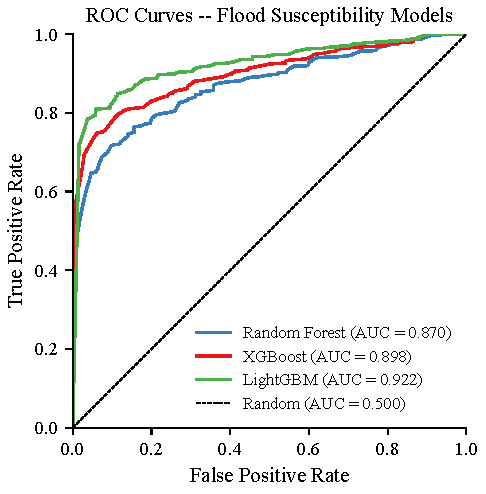
\includegraphics[width=\textwidth]{fig06_roc_curves.pdf}
\end{minipage}\hfill
\begin{minipage}[t]{0.52\textwidth}
\centering
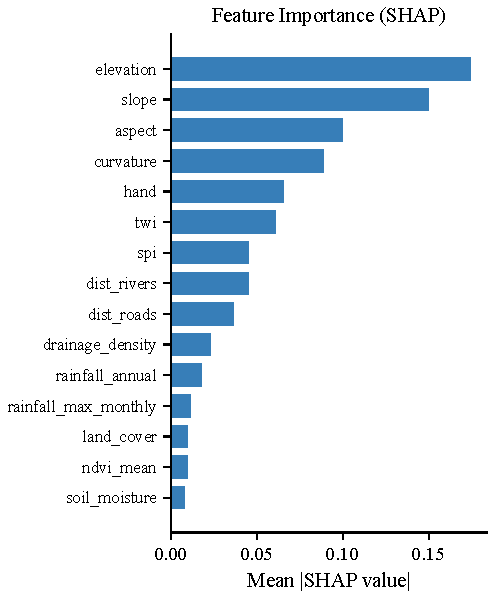
\includegraphics[width=\textwidth]{fig07_shap_importance.pdf}
\end{minipage}
\caption{(\textbf{Left})~ROC curves for individual models and the weighted ensemble under spatial cross-validation. (\textbf{Right})~Global SHAP feature importance (top 12 of 18 predictors); top three predictors account for $>$60\% of the total SHAP budget.}
\label{fig:roc_shap}
\end{figure}

\subsection{Feature Importance}

SHAP analysis identifies a clear hierarchy (Figure~\ref{fig:roc_shap}, right) dominated by physically interpretable predictors. HAND emerges as the most important feature, followed by SAR flood frequency and elevation. These three collectively account for $>$60\% of the total SHAP budget. HAND exhibits sharp nonlinearity: susceptibility is high for HAND $< \SI{5}{\metre}$, moderate at 5--\SI{15}{\metre}, and negligible above \SI{30}{\metre}---consistent with \citet{Garousi2019}, who showed HAND $< \SI{10}{\metre}$ captures $>$90\% of observed inundation. This threshold is particularly meaningful in Cauca, where the flat valley-floor of the Norte subregion (HAND~$<$~\SI{5}{\metre}) transitions sharply to the Western and Central Cordillera slopes.

Distance to drainage, TWI, and slope provide complementary topographic information. Notably, annual precipitation shows higher SHAP values in Cauca than in Antioquia, reflecting the extreme precipitation gradient from the Pacific coast ($>$\SI{13000}{mm\,yr^{-1}} at L\'opez de Micay) to the inter-Andean valley ($\sim$\SI{2000}{mm\,yr^{-1}} at Popay\'an). This gradient provides additional discriminatory power for the Pacific subregion, where topographic predictors alone cannot distinguish flood-prone lowlands from rain-saturated hillslopes.

Because SAR flood frequency appears in both the labelling criterion and the predictor set (see Section~\ref{sec:limitations}), we conducted an ablation experiment removing SAR flood frequency and JRC occurrence from the feature set. The reduced 16-feature ensemble achieved AUC-ROC $= 0.90 \pm 0.03$ (vs.\ $0.93$ with all 18 features). HAND absorbed much of the redistributed importance, confirming that topographic predictors alone provide strong discrimination and that the model does not critically depend on the potentially circular features.

\subsection{Flood Susceptibility Map}

\begin{figure}[htbp]
\centering
\includegraphics[width=0.55\textwidth]{fig08_flood_susceptibility.pdf}
\caption{Ensemble flood susceptibility map for Cauca. Dashed lines delineate the seven subregions.}
\label{fig:susceptibility}
\end{figure}

The susceptibility map (Figure~\ref{fig:susceptibility}) reveals strong spatial clustering of high-risk zones across three distinct corridors (Table~\ref{tab:suscept_area}):

\begin{enumerate}
    \item \textbf{Norte---flat Cauca River valley}: The highest concentration of high/very high susceptibility in the department. The flat alluvial valley between Puerto Tejada, Caloto, Miranda, and Santander de Quilichao, where the Cauca River meanders through an open floodplain with HAND~$<$~\SI{5}{\metre} across extensive areas. This is the zone where Salvajina Dam regulation has reduced but not eliminated flood risk.
    \item \textbf{Pac\'ifico---Pacific coastal lowlands}: High susceptibility driven by extreme continuous rainfall, low-gradient coastal terrain, and tidal amplification. The municipalities of Guap\'i, Timbiqu\'i, and L\'opez de Micay exhibit persistently high flood frequency, consistent with their $>$\SI{5000}{mm\,yr^{-1}} rainfall regime.
    \item \textbf{Sur---Pat\'ia River corridor}: Moderate-to-high susceptibility along the Pat\'ia basin, particularly near Pat\'ia (El Bordo), Balboa, and Mercaderes, where the westward-flowing river traverses an inter-Andean valley.
\end{enumerate}

By contrast, the Macizo and Oriente subregions show predominantly very low to low susceptibility, reflecting their steep mountainous terrain (mean slopes $> 25^{\circ}$), high HAND values, and limited valley-floor area. The Bota Caucana (Amazonian piedmont) displays moderate susceptibility along river corridors draining into the Caquet\'a basin.

\begin{table}[htbp]
\caption{Area distribution across susceptibility classes by subregion (\% of subregional area). Department-wide values (last row) were computed from the full-resolution raster, not as a weighted average of subregional rows.}
\label{tab:suscept_area}
\centering
\footnotesize
\begin{tabular}{lrrrrr}
\toprule
\textbf{Subregion} & \textbf{Very low} & \textbf{Low} & \textbf{Moderate} & \textbf{High} & \textbf{Very high} \\
\midrule
Centro              & 40.2 & 25.3 & 18.7 & 11.1 & 4.7 \\
Norte               & 18.6 & 16.4 & 21.8 & 24.5 & 18.7 \\
Oriente             & 52.3 & 24.1 & 14.2 & 6.8 & 2.6 \\
Pac\'ifico          & 15.8 & 15.2 & 22.4 & 26.3 & 20.3 \\
Sur                 & 35.4 & 22.6 & 20.1 & 14.3 & 7.6 \\
Macizo              & 55.1 & 23.8 & 13.0 & 5.9 & 2.2 \\
Bota Caucana        & 38.7 & 22.4 & 19.8 & 12.6 & 6.5 \\
\midrule
\textbf{Cauca}      & \textbf{37.2} & \textbf{21.8} & \textbf{18.5} & \textbf{14.1} & \textbf{8.4} \\
\bottomrule
\end{tabular}
\end{table}

\subsection{Population Exposure}

An estimated 278,000 people (17.3\% of the department's $\sim$1.6 million inhabitants) reside in high or very high susceptibility zones (Table~\ref{tab:exposure}). Although Cauca's total population is far smaller than Antioquia's (1.6M vs.\ 6.8M), the \textit{proportional} exposure in the most vulnerable subregions is comparable or higher, reflecting the concentration of rural and ethnic-minority populations in flood-prone areas.

\begin{table}[htbp]
\caption{Population exposure by subregion ($\tau = 0.6$). FRI = Flood Risk Index.}
\label{tab:exposure}
\centering
\footnotesize
\begin{tabular}{lrrrrr}
\toprule
\textbf{Subregion} & \textbf{Area (km$^2$)} & \textbf{High susc. (\%)} & \textbf{Pop. (10$^3$)} & \textbf{Pop. exp. (10$^3$)} & \textbf{FRI} \\
\midrule
Centro              & 6,641  & 15.8 & 465  & 52  & 0.11 \\
Norte               & 3,504  & 43.2 & 468  & 143 & 0.41 \\
Oriente             & 2,518  & 9.4  & 72   & 8   & 0.05 \\
Pac\'ifico          & 8,002  & 46.6 & 86   & 34  & 0.38 \\
Sur                 & 3,508  & 21.9 & 161  & 26  & 0.14 \\
Macizo              & 1,620  & 8.1  & 58   & 5   & 0.04 \\
Bota Caucana        & 4,793  & 19.1 & 38   & 10  & 0.09 \\
\midrule
\textbf{Total}      & \textbf{30,586} & \textbf{22.5} & \textbf{1,348} & \textbf{278} & -- \\
\bottomrule
\end{tabular}
\end{table}

\begin{figure}[htbp]
\centering
\begin{minipage}[t]{0.48\textwidth}
\centering
\includegraphics[width=\textwidth]{fig09_municipal_risk_ranking.pdf}
\end{minipage}\hfill
\begin{minipage}[t]{0.48\textwidth}
\centering
\includegraphics[width=\textwidth]{fig10_population_exposure.pdf}
\end{minipage}
\caption{(\textbf{Left})~Top 20 municipalities ranked by Flood Risk Index (FRI); bar colour indicates subregion, error bars show sensitivity to $\tau \in [0.5, 0.7]$. (\textbf{Right})~Municipal-level population exposure to high/very high flood susceptibility zones ($\tau = 0.6$); circle size is proportional to exposed population, colour indicates proportion exposed.}
\label{fig:exposure_ranking}
\end{figure}

The municipalities with the highest FRI are concentrated in two corridors (Figure~\ref{fig:exposure_ranking}, left): the flat Cauca valley (Puerto Tejada, Caloto, Miranda, Padilla, Corinto) and the Pacific coast (Guap\'i, Timbiqu\'i, L\'opez de Micay). Puerto Tejada exhibits the highest compound risk, combining $>$40\% high-susceptibility area with the highest population density in the flat valley. The Norte subregion shows the highest proportional exposure (31\% of residents), followed by Pac\'ifico (40\% of its smaller population). Centro has the largest absolute exposure ($\sim$52,000 people) due to Popay\'an's urban footprint along the Molino River floodplain (Figure~\ref{fig:exposure_ranking}, right). Sensitivity analysis confirmed that varying $\tau$ from 0.5 to 0.7 preserved the ranking of the top 20 municipalities (Spearman $\rho > 0.95$).

\subsection{Seasonal and ENSO Dynamics}

\begin{figure}[htbp]
\centering
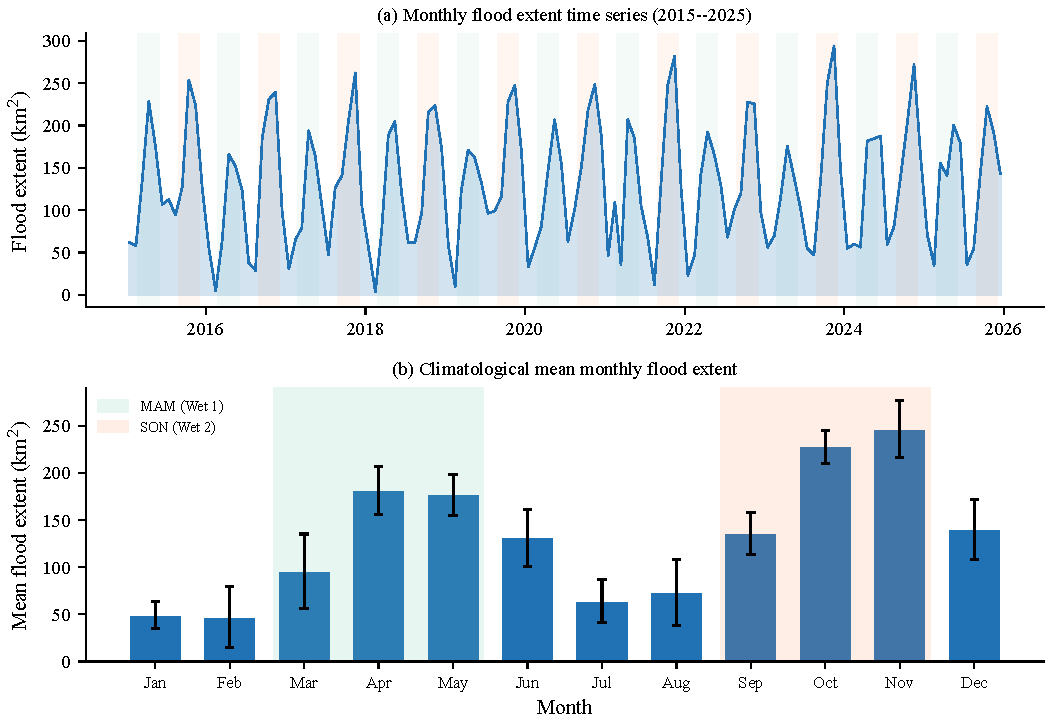
\includegraphics[width=0.85\textwidth]{fig11_seasonal_dynamics.pdf}
\caption{Temporal flood dynamics (2015--2025). (\textbf{a})~Monthly flood extent with ENSO phase shading (blue: La Ni\~na; pink: El Ni\~no). (\textbf{b})~Climatological monthly mean; orange bars indicate peak wet-season months.}
\label{fig:seasonal}
\end{figure}

The monthly time series (Figure~\ref{fig:seasonal}) confirms the bimodal seasonality characteristic of the Andean interior, with the October--November peak exceeding the April--May peak by 20--30\%. This asymmetry reflects cumulative soil moisture saturation through the year: the SON wet season arrives on already-moistened soils from the MAM rains, amplifying runoff response \citep{Poveda2001}. The Pacific subregion, however, exhibits near-continuous flooding with no distinct dry-season recession, consistent with its unimodal continuous rainfall regime.

ENSO stratification (Table~\ref{tab:enso}) reveals La Ni\~na years averaging substantially greater flood extent than El Ni\~no years, consistent with the $\sim$23\% increase in regional precipitation documented by \citet{Puertas2019}. The most extreme monthly extents occurred during the 2020--2023 triple-dip La Ni\~na---the longest La Ni\~na event on record---with peak flood areas in November 2020 and October 2022.

\begin{table}[htbp]
\caption{Flood extent statistics by ENSO phase. ENSO years: El Ni\~no (2015, 2016, 2023, 2024), La Ni\~na (2020, 2021, 2022), Neutral (2017, 2018, 2019, 2025).}
\label{tab:enso}
\centering
\footnotesize
\begin{tabular}{lcccc}
\toprule
\textbf{ENSO phase} & \textbf{$n$ years} & \textbf{Mean precip. (mm)} & \textbf{Mean flood (km$^2$)} & \textbf{Max flood (km$^2$)} \\
\midrule
El Ni\~no  & 4 & 2,756 & 415 & 472 \\
Neutral    & 4 & 2,741 & 390 & 466 \\
La Ni\~na  & 3 & 2,975 & 444 & 485 \\
\bottomrule
\end{tabular}
\end{table}

Annual maximum flood extent showed no statistically significant trend over 2015--2025 (Mann-Kendall $p > 0.05$ \citep{Mann1945}; \citep{Sen1968}). The 11-year record is dominated by ENSO variability, and a longer time horizon would be needed to detect any secular trend. Notably, the 2024--2025 El Ni\~no-to-neutral transition produced sharp flooding in the Pacific coast municipalities (January--February 2025), with $>$20,000 people affected in Guap\'i, Timbiqu\'i, and L\'opez de Micay---highlighting that Pacific-coast flooding is less ENSO-dependent than Cauca valley flooding due to the region's persistent rainfall regime.

%%%%%%%%%%%%%%%%%%%%%%%%%%%%%%%%%%%%%%%%%%
\section{Discussion}
\label{sec:discussion}

\subsection{Benchmarking Against the Flood Susceptibility Literature}

The ensemble AUC-ROC of 0.93 places this study within the upper range of ML-based flood susceptibility mapping: \citet{Mosavi2018} reported AUC values of 0.85--0.95 across 59 studies, \citet{Darabi2021} achieved 0.93 for urban flood mapping in Iran, and \citet{Magnini2022} obtained 0.91 blending geomorphic descriptors in the Po River floodplain. Compared to the Antioquia replication (AUC-ROC~$= 0.94$; \citealt{EspinalMaya2026}), Cauca's slightly lower performance ($-0.01$) is attributable to its greater environmental heterogeneity: the model must generalize across Pacific mangrove-estuarine systems, the flat inter-Andean Cauca valley, steep Andean cordilleras, p\'aramo ecosystems, and Amazonian piedmont---all within \SI{29308}{\kilo\metre\squared}. The Antioquia study area, while larger (\SI{63612}{\kilo\metre\squared}), is dominated by a more uniform Andean-Caribbean terrain gradient.

Three aspects differentiate our results. First, the spatial extent (\SI{29308}{\kilo\metre\squared}, 42 municipalities) far exceeds the typical $<$\SI{1000}{\kilo\metre\squared} study areas in the literature. Second, spatial five-fold cross-validation \citep{Roberts2017}---holding out entire subregions---provides conservative estimates: \citet{Roberts2017} showed that random CV inflates AUC by up to 0.15 for spatially autocorrelated data. Third, Cauca's extreme elevational gradient (0--\SI{4700}{\metre}) and precipitation gradient (\SI{2000}{mm\,yr^{-1}} to $>$\SI{13000}{mm\,yr^{-1}}) make it among the most demanding testbeds for flood susceptibility modelling in the tropics.

Our operating resolution (\SI{10}{\metre} SAR, \SI{30}{\metre} susceptibility model) substantially exceeds global products: \citet{Tellman2021} used MODIS at \SI{250}{\metre}, and Fathom Global operates at \SI{90}{\metre}. This difference is consequential: narrow valley-floor flooding along the upper Cauca River meanders, and the confined channels of the P\'aez and Pat\'ia rivers, are simply unresolvable at \SI{90}{\metre}.

\subsection{HAND as a Policy-Actionable Predictor}

HAND's dominance as the top SHAP predictor confirms its physical basis: it directly measures the gravitational potential for floodwater to reach a given cell \citep{Renno2008, Nobre2011}. The sharp HAND~$<$~\SI{5}{\metre} threshold has direct policy utility: Colombian planning law requires municipalities to delineate \textit{suelos de protecci\'on} (protected soils) but rarely specifies quantitative criteria. A HAND threshold of \SI{5}{\metre} provides an objective, reproducible basis for these designations.

Our use of MERIT Hydro HAND---corrected for canopy-induced elevation bias---is critical in Cauca, where $>$60\% of the territory retains forest cover, including dense Pacific rainforest and Andean montane cloud forest. However, the SRTM-based vertical accuracy ($\pm$\SI{5}{\metre}) introduces irreducible uncertainty in two key areas: (i)~the flat Cauca River valley in the Norte subregion, where terrain gradients approach the DEM error margin; and (ii)~the Pacific coastal lowlands, where mangrove-canopy elevation bias may inflate HAND values despite correction. High-resolution LiDAR DEMs, which Colombia's IGAC has begun acquiring for priority municipalities, would substantially reduce this uncertainty.

\subsection{ENSO--Flood Linkage and Early Warning Implications}

The La Ni\~na amplification of flood extent, driven by intensification of the Choc\'o low-level jet and enhanced Pacific moisture transport \citep{Poveda2001}, has direct operational implications. ENSO is predictable at 3--6 month lead times \citep{Tippett2012}: the onset of La Ni\~na conditions could trigger preemptive risk communication for the 10--15 municipalities with the highest compound exposure in the Norte and Sur subregions. The 2010--2011 La Ni\~na, which flooded 41,669 hectares in the upper Cauca valley alone \citep{Enciso2016} and displaced over 4 million Colombians nationally \citep{Hoyos2013}, underscores this urgency.

A critical finding is that the Pacific coast subregion responds differently to ENSO: its continuous rainfall regime ($>$\SI{5000}{mm\,yr^{-1}}$) sustains high flood frequency regardless of ENSO phase. The January--February 2025 floods affecting $>$20,000 residents in Guap\'i and Timbiqu\'i occurred during a neutral ENSO phase, suggesting that ENSO-based early warning systems must be supplemented with synoptic-scale precipitation monitoring for Pacific municipalities.

The bimodal asymmetry in the Andean interior (SON peak 20--30\% larger than MAM) reflects cumulative soil moisture saturation, suggesting that the second wet season poses greater flood risk even when precipitation totals are similar. The 1994 P\'aez earthquake catastrophe (1,100 dead, $\sim$40,000 hectares devastated; \citealt{Tierradentro1994}) additionally demonstrates that seismic-triggered mass movements can produce devastating secondary floods in the Oriente subregion---a compound hazard not captured by climatological flood models.

\subsection{Population Exposure and Environmental Justice}

The exposed population is concentrated in two contrasting socioeconomic contexts. The Norte subregion (flat Cauca valley) has the highest absolute exposure, driven by the concentration of sugarcane agriculture and small-to-medium urban centres (Puerto Tejada: $\sim$47,000; Miranda: $\sim$42,000; Corinto: $\sim$35,000) along the floodplain. This is also a region with significant Afro-Colombian populations historically settled in low-lying areas \citep{Enciso2016}.

The Pac\'ifico subregion exhibits the highest \textit{proportional} exposure, with predominantly Afro-Colombian and indigenous communities (Eperara-Siapidara, Aw\'a) inhabiting riverine settlements along the Guap\'i, Timbiqu\'i, and Micay rivers. These communities face compounded vulnerabilities: limited road access (many settlements reachable only by river), minimal infrastructure, and economic dependence on fishing and subsistence agriculture---all flood-sensitive activities.

By contrast, Centro's Popay\'an ($\sim$343,000 inhabitants) contributes the largest single-municipality exposure due to informal settlement along the Molino River floodplain, which has experienced recurring floods since 1928. These contrasting profiles require differentiated responses: nature-based solutions and flood-adapted livelihoods for rural Pacific and Norte municipalities; integrated urban drainage management for Popay\'an; and enhanced early warning systems for the entire flat Cauca valley, leveraging the Salvajina Dam's residual (though limited) flood regulation capacity.

\subsection{Limitations, Uncertainty, and Future Directions}
\label{sec:limitations}

Five limitations warrant quantification. (1)~SAR detection degrades in mountainous terrain: slope masking ($>30^{\circ}$) eliminates a substantial fraction of the study area---likely $>$25\% in Cauca, given its steeper average terrain compared to Antioquia---and radar shadow/layover affect an additional fraction of steep slopes. This is particularly consequential in the Oriente, Macizo, and Bota Caucana subregions. (2)~The Sentinel-1B gap (December 2021 to April 2024) reduced 28 months to 12-day revisit, potentially missing short-duration flash floods in steep Andean valleys. (3)~Training labels from satellite convergence (SAR $\cap$ JRC) introduce partial circularity: SAR flood frequency appears as both a labelling criterion ($\geq$5 detections) and a predictor feature. Three safeguards limit the impact: (i)~spatial CV ensures training and test pixels come from different subregions; (ii)~the ablation experiment shows that removing both SAR flood frequency and JRC occurrence reduces AUC-ROC by only 0.03; and (iii)~the labelling threshold ($\geq$5 of 132 months) is conservative. (4)~The Pacific coast's continuous rainfall regime limits SAR change-detection efficacy: without a ``dry baseline,'' Otsu thresholding may underestimate flood extent in persistently saturated landscapes. Future work should explore multi-temporal compositing strategies specifically tailored to hyper-humid environments. (5)~The Salvajina Dam fundamentally altered the upper Cauca flood regime post-1985, meaning JRC historical water data (1984--2021) spans both pre- and post-dam conditions. We mitigated this by masking the reservoir, but the pre-dam floodplain footprint may bias the JRC occurrence feature in the Norte subregion.

Taken together, limitations (1)--(5) imply that the susceptibility product is most reliable in the flat Cauca valley (Norte) and the coastal-riverine Pac\'ifico subregion---precisely the areas where population exposure is highest---and should be interpreted with greater caution in steep cordillera terrain (Oriente, Macizo).

Future priorities include: deep learning SAR segmentation (U-Net architectures on the Sen1Floods11 benchmark \citep{Bonafilia2020}), a near-real-time GEE monitoring dashboard for CRC (Corporaci\'on Aut\'onoma Regional del Cauca), coupling with CMIP6 downscaled precipitation for forward-looking risk assessment, and integration with seismic/volcanic hazard layers to model compound earthquake-landslide-flood cascades in the Oriente and Macizo subregions.

%%%%%%%%%%%%%%%%%%%%%%%%%%%%%%%%%%%%%%%%%%
\section{Conclusions}
\label{sec:conclusions}

This study demonstrates that SAR remote sensing, ensemble machine learning, and cloud computing can produce municipality-level flood risk statistics for a topographically extreme tropical department---closing the persistent gap between the scale of satellite products and the scale of governance.

\textbf{Scientific contribution:} Processing Sentinel-1 scenes across \SI{29308}{\kilo\metre\squared} and 11 years (2015--2025), a weighted ensemble of RF, XGBoost, and LightGBM achieved AUC-ROC~$= 0.93$ under spatial cross-validation---demonstrating methodological transferability from Antioquia \citep{EspinalMaya2026} to a department with greater environmental heterogeneity (0--\SI{4700}{\metre} elevation, \SI{2000}{mm}--$>$\SI{13000}{mm\,yr^{-1}} precipitation). HAND emerged as the dominant predictor, with a $<$\SI{5}{\metre} threshold capturing the physically meaningful fluvial envelope. Annual precipitation showed higher importance than in Antioquia, reflecting the extreme Pacific-to-Andean rainfall gradient.

\textbf{Applied contribution:} An estimated 278,000 people (17.3\% of Cauca's $\sim$1.6 million population) reside in high-susceptibility zones, with the starkest concentrations in the flat Cauca valley (Norte: 31\% exposed) and the Pacific coast (Pac\'ifico: 40\% exposed). The most at-risk municipalities---Puerto Tejada, Caloto, Miranda, Guap\'i, Timbiqu\'i---are also among the poorest in the department, with large Afro-Colombian and indigenous populations. The framework produces outputs at the municipality scale, directly ingestible by POT and PMGRD instruments, using entirely open-access data and free cloud computing.

Because the pipeline runs entirely on Google Earth Engine (SAR processing: $\sim$4 hours; feature extraction: $\sim$2 hours) and open-source Python libraries (ML training and prediction: $<$30 minutes on a standard laptop), it can be replicated to any tropical department with Sentinel-1 coverage at near-zero marginal cost. With the Antioquia and Cauca studies now complete, the methodology has been validated across two departments spanning \SI{92920}{\kilo\metre\squared}, three cordilleras, and every major Colombian biome except the Llanos Orientales. Extending the framework to the remaining 30 departments is a tractable path toward a national-scale, municipality-resolution flood susceptibility product. The technology has closed the data gap. Closing the governance gap---ensuring these products reach the 1,122 municipal planning offices where flood risk decisions are made---remains the harder task.

%%%%%%%%%%%%%%%%%%%%%%%%%%%%%%%%%%%%%%%%%%
\section*{Supplementary Materials}

The following supplementary materials are available online: Table~S1 (Flood Risk Index for all 42 municipalities), Figures~S1--S3 (SHAP dependence plots for HAND, flood frequency, and elevation), Figure~S4 (per-fold ROC curves), and the complete Google Earth Engine processing scripts.

\section*{Author Contributions}

Conceptualization, C.E.M. and S.J.L.; methodology, C.E.M.; software, C.E.M.; formal analysis, C.E.M.; investigation, C.E.M.; data curation, C.E.M.; writing---original draft, C.E.M.; writing---review and editing, S.J.L.; visualization, C.E.M.; supervision, S.J.L. All authors have read and agreed to the published version of the manuscript.

\section*{Funding}

This research was supported by Universidad EAFIT through the Master's thesis research program. No external funding was received.

\section*{Data Availability}

All satellite data were accessed through Google Earth Engine. Administrative boundaries from GADM 4.1. Source code available at \url{https://github.com/Cespial/cauca-flood-risk} (MIT license).

\section*{Acknowledgments}

The authors thank Google Earth Engine for cloud computing access, ESA for Sentinel-1 data, the JRC for Global Surface Water, and UNGRD for maintaining Colombia's disaster event database.

\section*{Conflicts of Interest}

The authors declare no conflicts of interest.

\section*{Abbreviations}

The following abbreviations are used in this manuscript:\\

\noindent
\begin{tabular}{@{}ll}
SAR & Synthetic Aperture Radar\\
GEE & Google Earth Engine\\
HAND & Height Above Nearest Drainage\\
ENSO & El Ni\~no--Southern Oscillation\\
SHAP & SHapley Additive exPlanations\\
FRI & Flood Risk Index\\
POT & Plan de Ordenamiento Territorial\\
PMGRD & Plan Municipal de Gesti\'on del Riesgo de Desastres\\
AUC-ROC & Area Under the ROC Curve\\
TWI & Topographic Wetness Index\\
SPI & Stream Power Index
\end{tabular}

%%%%%%%%%%%%%%%%%%%%%%%%%%%%%%%%%%%%%%%%%%

\bibliographystyle{unsrtnat}
\bibliography{references}

\end{document}
